\documentclass[tikz]{standalone}

\begin{document}
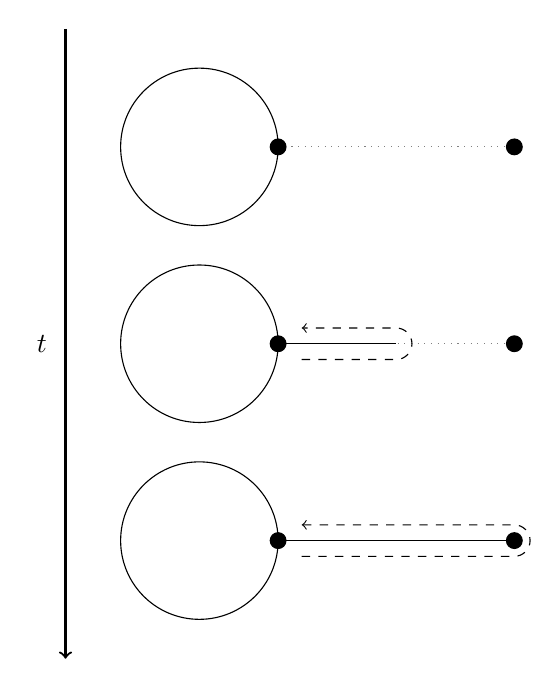
\begin{tikzpicture}

% The time axis
\draw[color=black,->,thick] (-1.7,1.5) -- (-1.7,-6.5);
\node at (-2,-2.5) {\(t\)};

% The circular paths
\draw[color=black] (0,0) circle (1);
\draw[color=black] (0,-2.5) circle (1);
\draw[color=black] (0,-5) circle (1);

% The Cs
\draw[color=gray,dotted] (1,0) -- (4,0);
\draw[color=gray,dotted] (1,-2.5) -- (4,-2.5);
\draw[color=gray,dotted] (1,-5) -- (4,-5);

% The x_0 points
\filldraw[color=black] (1,0) circle (.1);
\filldraw[color=black] (1,-2.5) circle (.1);
\filldraw[color=black] (1,-5) circle (.1);

% The x points
\filldraw[color=black] (4,0) circle (.1);
\filldraw[color=black] (4,-2.5) circle (.1);
\filldraw[color=black] (4,-5) circle (.1);

% The evolving path
\draw[color=black] (1,-2.5) -- (2.5,-2.5);
\draw[color=black] (1,-5) -- (4,-5);

% The evolving arrow
\draw[color=black,dashed,->] (1.3,-2.7) -- (2.5,-2.7) arc (-90:90:.2) -- (1.3,-2.3);
\draw[color=black,dashed,->] (1.3,-5.2) -- (4,-5.2) arc (-90:90:.2) -- (1.3,-4.8);

\end{tikzpicture}
\end{document}
